\documentclass[svgnames,smaller,table]{beamer}
\usepackage{multirow}
\usepackage{tikz}
\usefonttheme[onlymath]{serif}

\usepackage{listings}
% Configura o listings
\lstset{
  %  basicstyle=\footnotesize,\small,...\tiny
  basicstyle=\ttfamily\scriptsize,
  commentstyle=\color{mygreen},
  numbers=left,
  stepnumber=1,
  showstringspaces=false,
  tabsize=2,
  breaklines=true,
  breakatwhitespace=false
 columns=fixed,
 fontadjust=true,
 basewidth=0.5em
}


\usetheme{lthn}
\setbeamercolor*{normal text}{fg=black}
% -----------------------------------------------------------------------------------------------------------------

\title[Slide]{The Use of Serpent at the LTHN/CDTN}
\author{Vitor Vasconcelos A. Silva}
\date{\today}
\institute{%
  LTHN - Thermal-hydraulics and Neutronics Laboratory
  \par
  Reactors Technology Service - CDTN/CNEN}

\begin{document}

%-------------------------------------------------
\begin{frame}
\titlepage
\end{frame}

%-------------------------------------------------
\begin{frame}
  \frametitle{Summary}
  \tableofcontents%[pausesections]
\end{frame}


\section{CDTN}
%-------------------------------------------------
\begin{frame}
  \frametitle{CDTN}
  \framesubtitle{Nuclear Technology Development Center}
  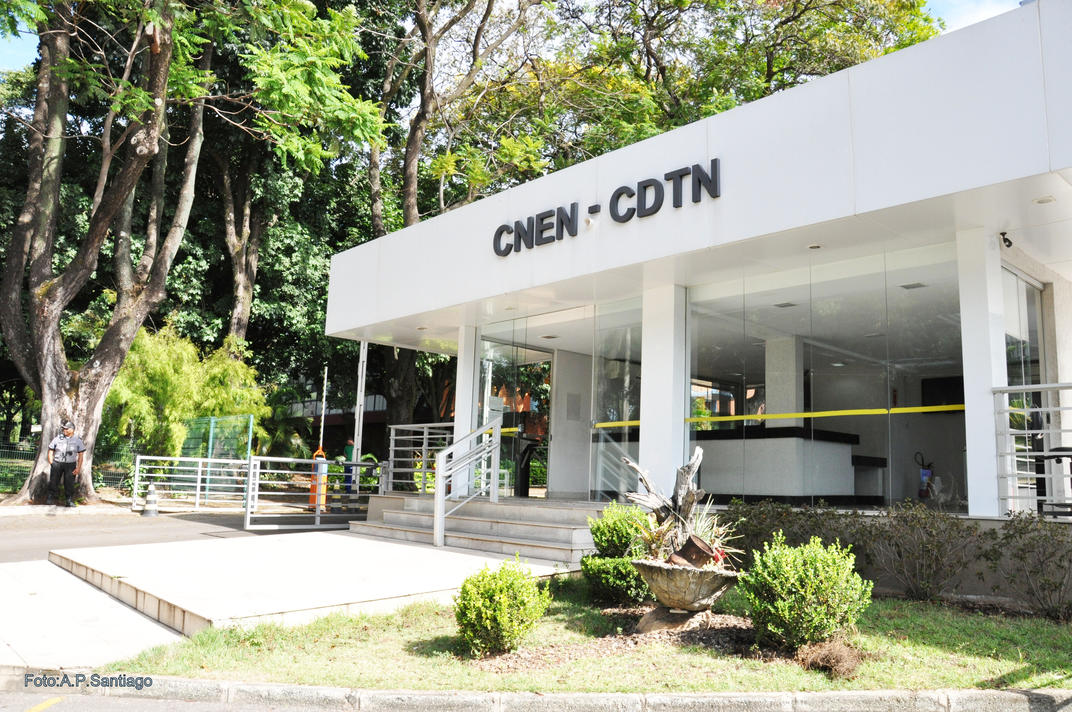
\includegraphics[scale=0.07]{figuras/portaria1_CDTN.jpg}
\end{frame}

%-------------------------------------------------
\begin{frame}
  \frametitle{CDTN}
  \framesubtitle{Nuclear Technology Development Center}
  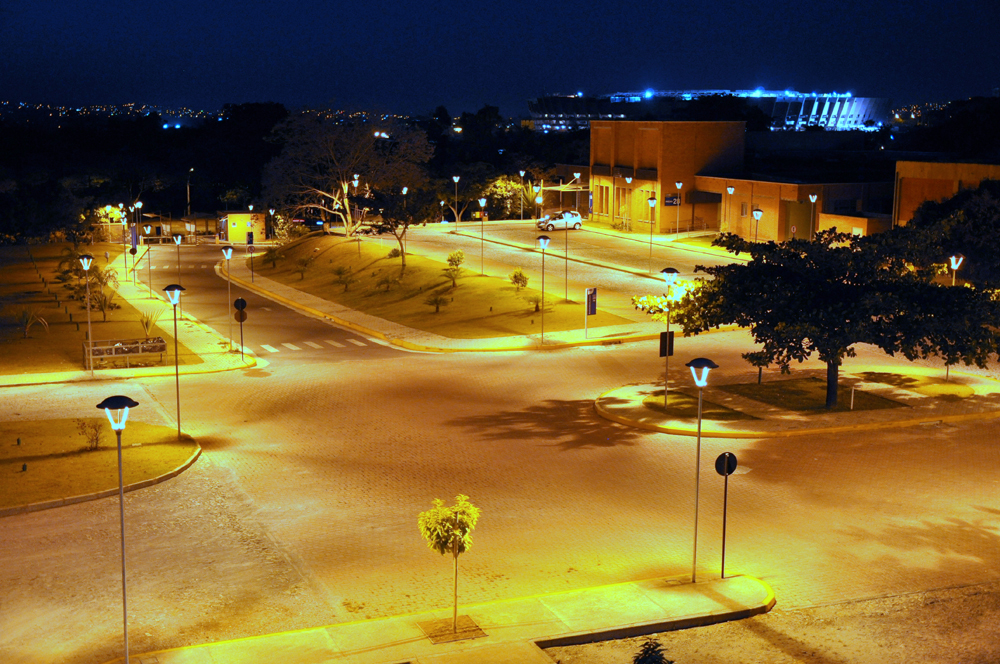
\includegraphics[scale=1.3]{figuras/predio_28_noite.jpg}
\end{frame}

%-------------------------------------------------
\begin{frame}
  \frametitle{CDTN}
  \framesubtitle{Nuclear Technology Development Center}
  \begin{itemize}
  \item Founded in 1952 as IPR (Radioactive Research Institute), part of
    Minas Gerais Federal University.
  \item In 1960, TRIGA Mark 1 reactor inaugurated - first criticality.
  \item Many areas...
    \item Neutronics + thermal....
  \end{itemize}
\end{frame}


\section{Thermal-Hydraulics and Neutronics Lab - LTHN}
%-------------------------------------------------
\begin{frame}
  \frametitle{Thermal-Hydraulics and Neutronics Lab - LTHN}
  \begin{center}
    Figura
    %    \includegraphics[scale=0.2]{figuras/extrator-poco.jpg}
  \end{center}
\end{frame}

%-------------------------------------------------
\begin{frame}
  \frametitle{Thermal-Hydraulics and Neutronics Lab - LTHN}
  \framesubtitle{Main activities}
  \begin{center}
    \begin{itemize}
    \item Andre
    \item Daniel
    \item Graici
    \item Vitor
    \end{itemize}
  \end{center}
\end{frame}

\section{Monte Carlo simulation work}
%-------------------------------------------------
\begin{frame}
  \frametitle{Monte Carlo simulation work}
  \framesubtitle{Serpent2 use}
  \textbf{Monte Carlo}
    \begin{itemize}
    \item RMB...
    \item Novos combustiveis...
    \item Fusao...
    \end{itemize}
    \vspace{10px}
  \textbf{Algo aqui?}
    \begin{itemize}
    \item bla
    \end{itemize}
\end{frame}

\subsection{Tiago - acoplamento}
%-------------------------------------------------
\begin{frame}
  \frametitle{OpenFOAM + Serpent2 coupling}
  \framesubtitle{Pin simulation using coarse mesh}
  \begin{center}
%    \includegraphics[scale=0.2]{figuras/esquema.png}
    Outra figura?
  \end{center}
\end{frame}

\begin{frame}
  \frametitle{OpenFOAM + Serpent2 coupling}
  \framesubtitle{Details}
  \begin{center}
%    \includegraphics[scale=0.2]{figuras/esquema.png}
    Outra figura?
  \end{center}
\end{frame}

\begin{frame}
  \frametitle{OpenFOAM + Serpent2 coupling}
  \framesubtitle{Results}
  \begin{center}
%    \includegraphics[scale=0.2]{figuras/esquema.png}
    Outra figura?
  \end{center}
\end{frame}

\begin{frame}
  \frametitle{OpenFOAM + Serpent2 coupling}
  \framesubtitle{Problems}
  \begin{center}
%    \includegraphics[scale=0.2]{figuras/esquema.png}
    Outra figura?
  \end{center}
\end{frame}
% END SUBSECTION----------------------------------

\subsection{Graici - queima}
%-------------------------------------------------
\begin{frame}
  \frametitle{Neutron Extractor}
  \framesubtitle{View}
  \begin{center}
%    \includegraphics[scale=0.2]{figuras/extrator1-original.jpg}
    Figura de novo.
  \end{center}
\end{frame}

\subsection{Graici - fusao}
%-------------------------------------------------
\begin{frame}
  \frametitle{Neutron Extractor}
  \framesubtitle{Closer view}
  \begin{center}
%    \includegraphics[scale=0.2]{figuras/extrator-zoom.jpg}
    Chega de figuras
  \end{center}
\end{frame}

%-------------------------------------------------
%\begin{frame}
%  \frametitle{Neutron Extractor}
%  \framesubtitle{Technical aspects related to neutrongraphy}
%    \begin{itemize}
%    \item Collimation ratio: \scalebox{1}{$\left(\frac{L}{D}\right)=\frac{460cm}{10cm}=46$}
%    \item Neutron to gamma ratio: \scalebox{1.5}{$\frac{n}{\gamma}$} $ = 153 \times 10^4 (mR)^{-1}.cm^{-2}$ \textsuperscript{[}\footnote{A. L. Costa, 2003}\textsuperscript{]} 
%    \item Only one report on thermal/epithermal neutrons (Cd) ratio: at 3.6 meters over reactor's graphite reflector it is $27$. (Information only) 
%    \end{itemize}
%    \vspace{10px}
%\end{frame}

\section{Conclusions}
%-------------------------------------------------
\begin{frame}
  \frametitle{Conclusions}
  \framesubtitle{And some future intentions}
  Roughly, half of the activities of neutronic modelling and simulation at the LTHN are done using Serpent2.
\end{frame}



%-------------------------------------------------
% FIM
%-------------------------------------------------
\begin{frame}
 \vfill
  \begin{beamercolorbox}[center]{title}
     \Huge{Thank you!}
  \end{beamercolorbox}
  \vfill
\end{frame}


\end{document}

